\documentclass[../thesis.tex]{subfiles}
\begin{document}

\chapter{Experiments}
\label{ch:experiments}
In this section, the frame field generation applied to a cube mesh
with some different metrics is discussed.
\emph{Setup:} We store the associated matrices of the metric field at each vertex of the
tet mesh. The cube has corners at $(0,0,0)$ and $(1,1,1)$. The frame field optimization is run to depth 3.

To start, we apply the constant metric  $g^{1/2}=\mathrm{diag}(1,1,1)$
everywhere. The rotation coefficients $R$ are the identity matrix everywhere, as the metric does not twist or squish the space within the field.
The result is the boundary aligned frame field with no singularities, as the energy can be minimised to zero if the frames are constant. Figure \ref{fig:image1} shows the mesh used to store the metric
and the resulting constant frame field.
\begin{figure}[htb]
    \centering
    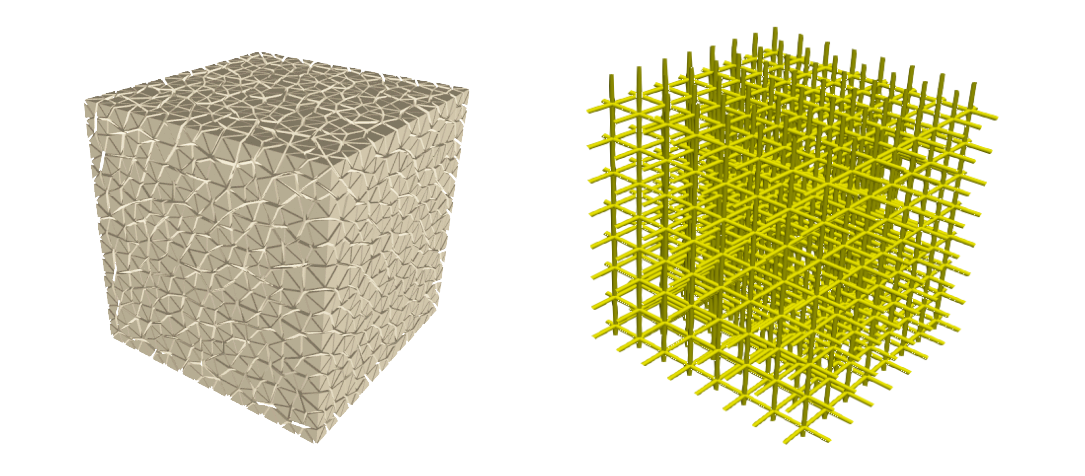
\includegraphics[width=\textwidth]{figures/image1}
    \caption{Left: The mesh used to store the metric field. Right: Constant metric everywhere which gives the boundary aligned constant frame field with no singularities.}
    \label{fig:image1}
\end{figure}

To further validate the frame field generation, we divide along the cube along
the $z$-axis into three equally sized parts.
The function to attach the metric to the vertices is then defined as
$$g^{1/2}(z) = \begin{cases}
    \mathrm{diag}(1,1,1) &0 < z < 1/3 \\
    \mathrm{diag}(27z-8,1,27z-8) &1/3 < z < 2/3 \\
    \mathrm{diag}(10,1,10) &2/3 < z < 1 \\
\end{cases}$$
The metric is constant in the $y$-axis and constant-linear-constant in the $x,z$-axis.
Thus, the rotation coefficients are only of the form
$$\begin{pmatrix}
    \cos (\alpha) & 0 & \sin(\alpha) \\
    0 & 1 & 0 \\
    -\sin(\alpha) & 0 & \cos(\alpha)
\end{pmatrix}$$
for some angle $\alpha$.
The result is depicted in figure \ref{fig:image2}.
\begin{figure}[htb]
    \centering
    \def\svgwidth{\textwidth}
    \input{figures/Zeichnung.pdf_tex}
    \caption{(a) The varying $g^{1/2}_{00}$ component along the $z$-axis. Visible is how
    the streamlines of the frame field only change in the middle third (b) and how the frames do not change along the $y$-axis (c).
    The singularities (d) are only points when taking a slice along the $y$-axis.}
    \label{fig:image2}
\end{figure}





\begin{itemize}
    \item As a sanity check, we start with the constant metric everywhere.
    
    
    
    constant metric everywhere -> no singularities
    \item linearly increasing metric in z-axis, isotropic scaling
    \item 2d example anisotropic scaling, constant-linear-constant
    \item larger cubes at the edges of the cube, isotropic scaling
\end{itemize}

\end{document}